\section{Lower bound instance}\label{sec:4:instance}

This section contains an explicit graphical representation of the
lower bound of $45/33$ for $3$ bins.

\begin{figure}
  \centering
  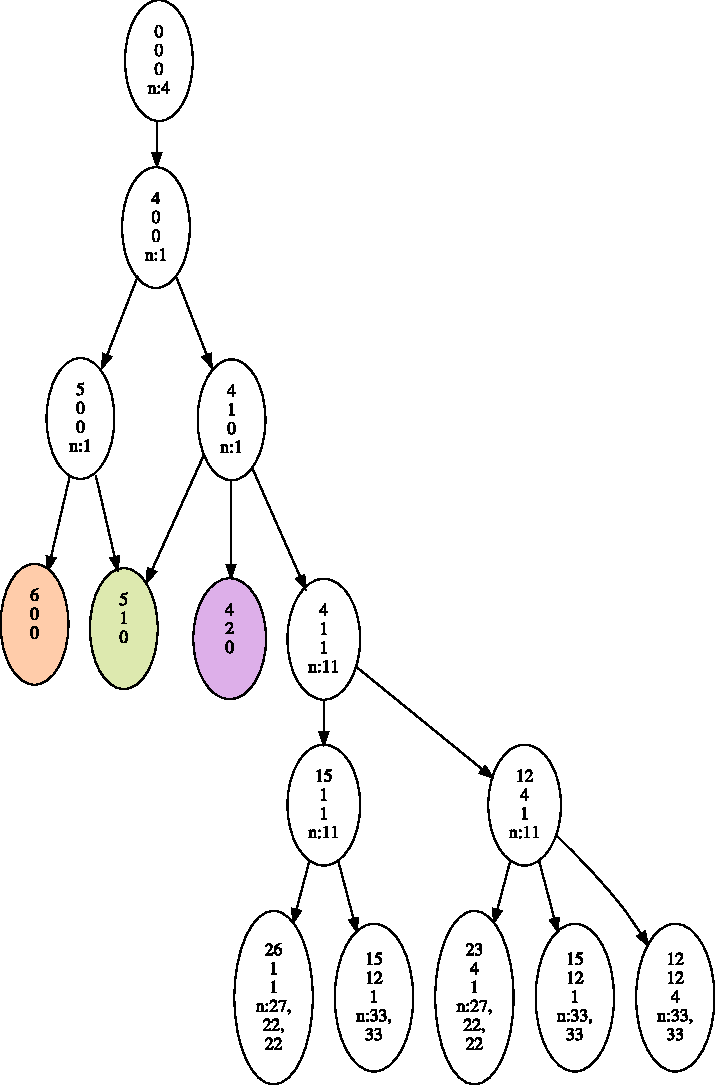
\includegraphics[scale=0.65]{img/big_picture.pdf}
  \caption{The beginning moves of the $45/33$ lower bound, scaled so
      that $T = 33$ and $S = 45$. The vertices contain the current
      loads of all three bins, and a string \texttt{n: $i$} with $i$
      being the next item presented by the \adversary. If there are
      several numbers after \texttt{n:}, the items are presented in
      the given order, regardless of packing by the player \algo. The coloured vertices are expanded in later figures.}
\end{figure}
\newpage
\begin{figure}
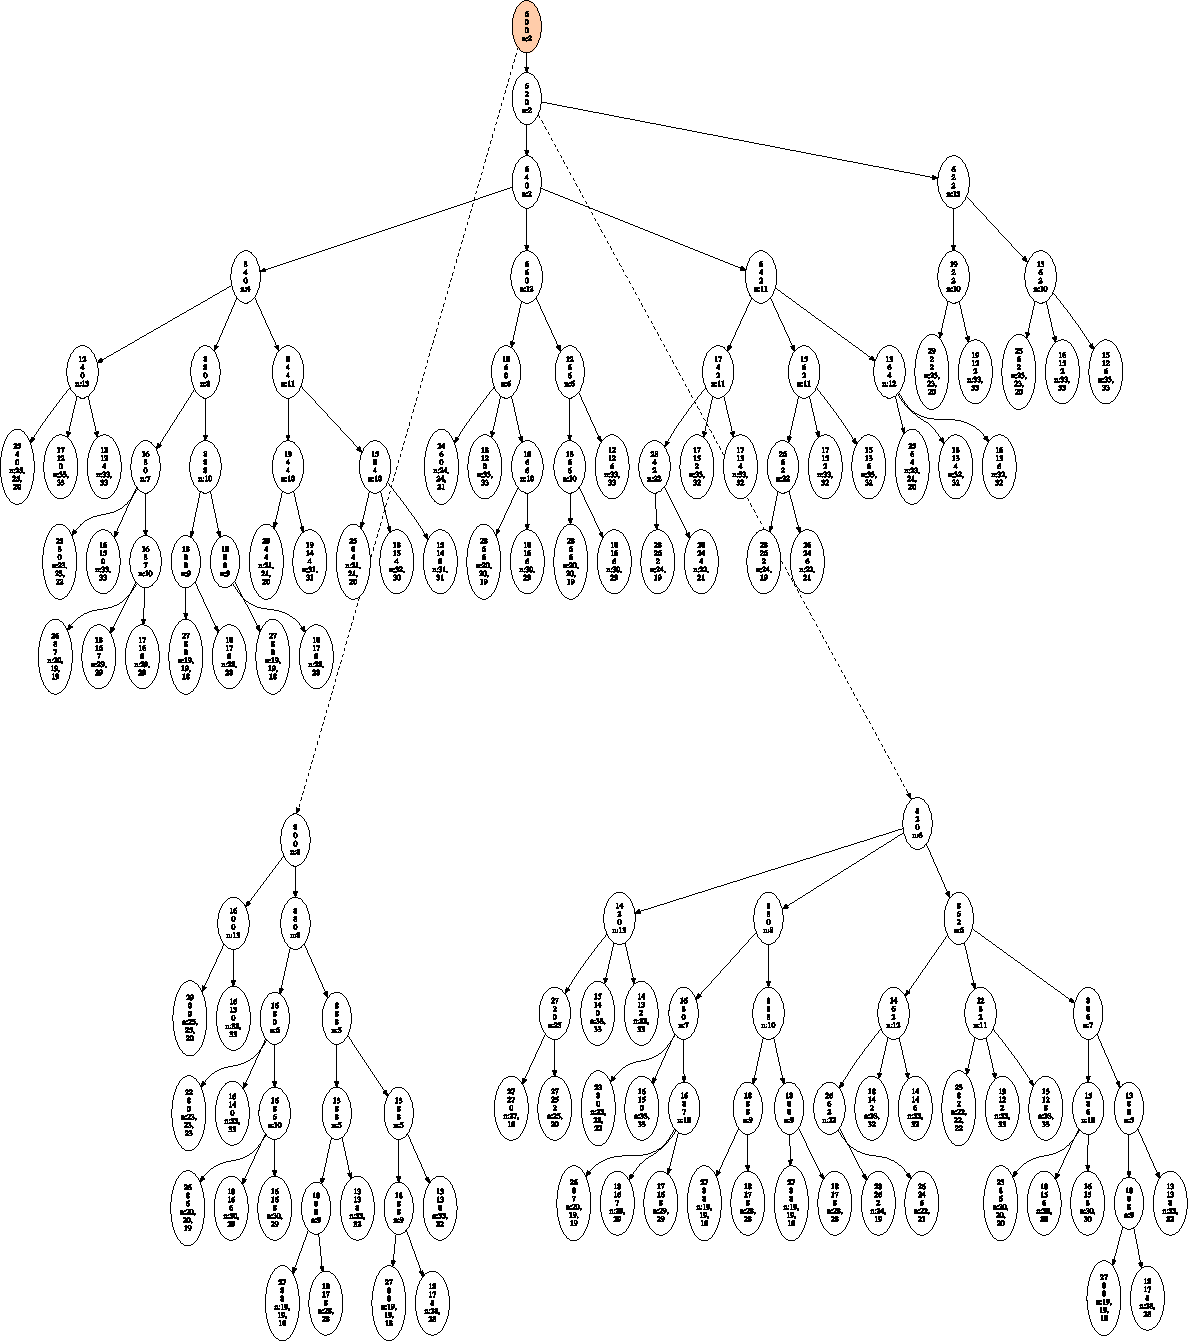
\includegraphics[scale=0.6]{img/6-0-0.pdf}
\caption{Game tree for the lower bound of $45/33$, starting with the bin configuration $(6,0,0,\{4,1,1\})$.}
\end{figure}

\begin{figure}
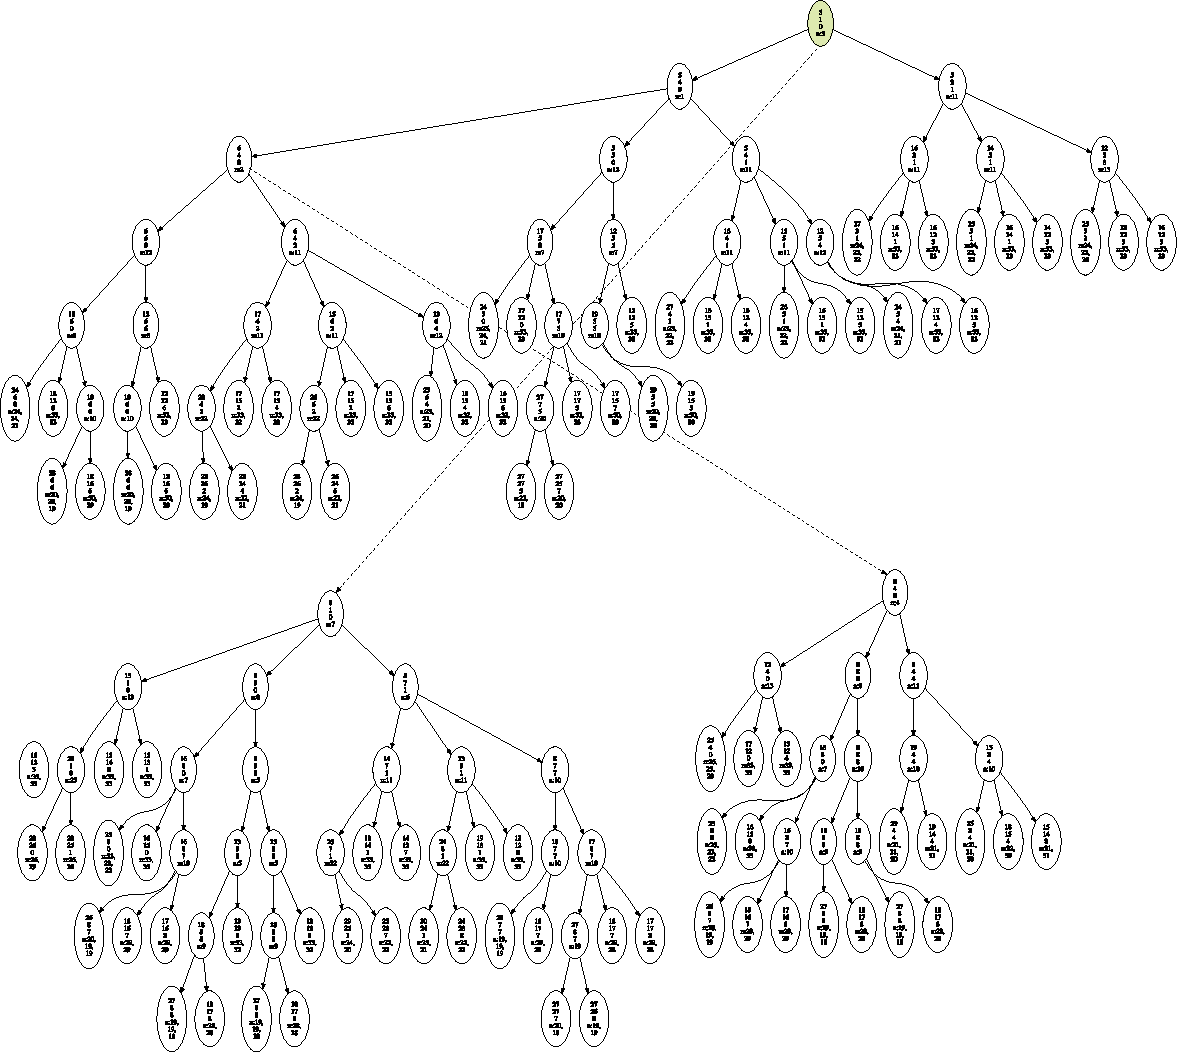
\includegraphics[scale=0.6]{img/5-1-0.pdf}
\caption{Game tree for the lower bound of $45/33$, starting with the bin configuration $(5,1,0,\{4,1,1\})$.}
\end{figure}

\begin{figure}
  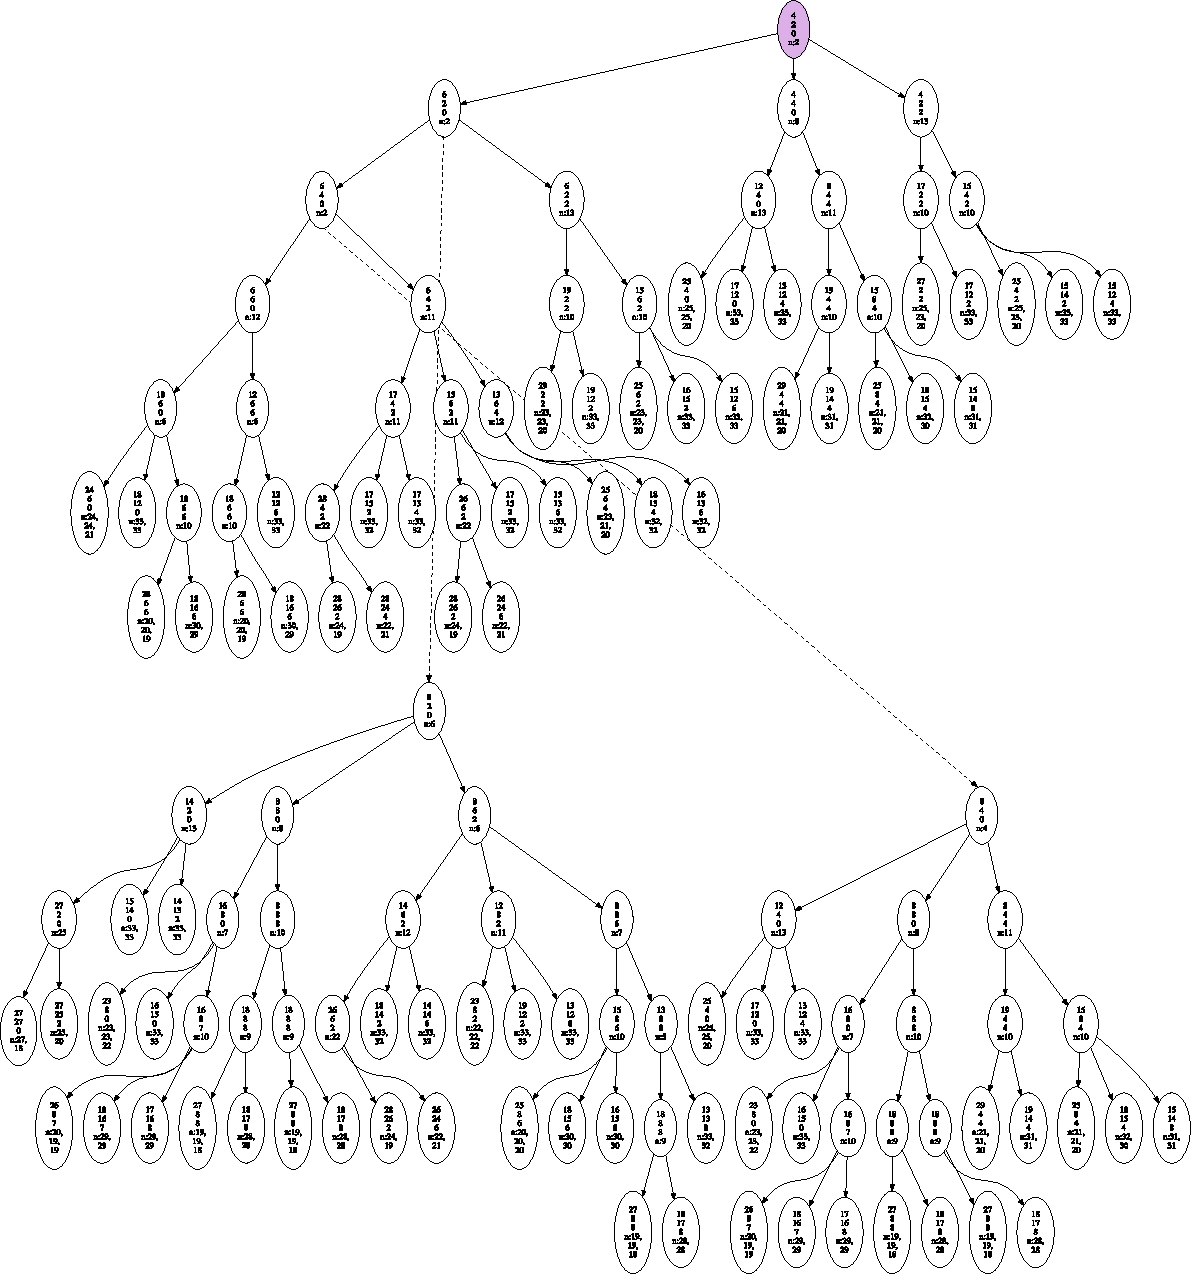
\includegraphics[scale=0.6]{img/4-2-0.pdf}
  \caption{Game tree for the lower bound of $45/33$, starting with the bin configuration $(4,2,0,\{4,1,1\})$.}
\end{figure}